\documentclass[11pt]{article}
\usepackage{icmlko}
\begin{document}

\title{이미 알고 있었다 --- 도메인 원핫이 나르는 정보는 표시자 열에 다 들어 있다}
\author{월드모델 실험실}
\date{노트 404 · 2026년 8월 1일}
\maketitle

\begin{abstract}
노트 401이 도메인 원핫의 값을 설명하지 못한 채 닫혔다 --- 크기
($\rho{=}{+}0.26$), 상호작용($+0.02$), 축 결측($+0.07$) 셋이 다 죽었다.
노트 403이 실마리를 하나 남겼다: \emph{팝업은 공유 축에 얹혀 가는
도메인이다.} 그렇다면 물어야 할 것은 ``원핫이 무엇을 더 아는가''다.

F18 의 자질 만드는 자리(\texttt{\_feat})는 축마다 \textbf{값 열 하나와
관측 표시자 열 하나}를 낸다 --- 축 열일곱이면 서른넷이다. 도메인마다 가진
축이 다르니 그 표시자 무늬가 \textbf{이미 도메인을 부르고 있을} 수 있다.
학습 18{,}540행에서 쟀다.

\begin{center}
\begin{tabular}{lrr}
\hline
 & 표시자 무늬 순도 & 드롭아웃 손해 \\
\hline
아홉 도메인(게임·모바일·세계애니·시장팝업 & \multirow{2}{*}{$\mathbf{1.000}$}
 & $-0.1039 \sim +0.0276$ \\
\quad ·아이돌·애니·웹툰·팝업·펀딩) & & \\
\hline
만화 & $0.204$ & $-0.0052$ \\
도서 & $\mathbf{0.000}$ & $-0.0053$ \\
\hline
\end{tabular}
\end{center}

\textbf{열한 도메인 중 아홉이 순도 1.000 이다} --- 표시자 무늬만 보면 어느
도메인 행인지 유일하게 정해진다. \textbf{원핫은 정보를 하나도 안 더한다.}
그런데도 빼면 아이돌이 $0.104$, 게임이 $0.057$ 을 잃는다. 그리고 정보를
못 주는 유일한 둘(도서·만화)이 \textbf{제일 적게} 잃는다 --- 순도와 손해의
순위상관은 $\rho = -0.067$ 이다.
\end{abstract}

\section{무늬는 왜 도메인을 부르는가}

도메인마다 붙는 축이 다르다(그림 나). 아이돌은 한터·위키·달력 축을 갖고
추세 축이 없다. 게임은 위키·추세를 갖고 태그 축이 없다. 팝업은 다섯 축뿐이다.
이 ``가진 축의 집합''이 곧 표시자 무늬이고, 무늬 일흔 개가 열한 도메인을
거의 그대로 가른다.

겹치는 둘은 \textbf{도서와 만화}다 --- 둘 다 같은 축 묶음을 쓰고, 도서는
\textbf{제 무늬를 하나도 독차지하지 못한다}(순도 0.000). 두 도메인이 축
구성에서 형제라는 뜻인데, 그 둘이 원핫을 빼도 거의 안 흔들린다.

\section{그러면 원핫은 무엇을 파는가}

정보가 아니다. 남는 후보는 \textbf{편의}다 --- 나무가 ``이 행은 아이돌이다''를
쓰려면 원핫이 있을 땐 갈림 \textbf{하나}면 되고, 없을 땐 표시자 서른네 열의
\textbf{논리곱}을 깊이를 써서 다시 지어야 한다. 자질 공간은 같아도 그 공간을
쓰는 값이 다르다.

\textbf{사전 등록했다}: 편의가 맞으면 \textbf{깊이가 원핫을 대신할 수 있어야
한다}. 원핫 없는 팔에서 깊이를 올리면 아이돌·게임이 회복하고, 원핫 있는
팔에서는 평평하다(노트 272가 이미 깊이를 죽였다). \textbf{상호작용이
예측이다.} 두 팔 다 평평하면 편의도 아니고, 원핫이 파는 것은 자질 공간의
성질이 아니라 부스팅 경로의 성질이다.

\section{재는 방식의 한계}

순도는 \textbf{학습 행}에서 \textbf{정확히 같은 무늬}로만 쟀다. 무늬가
달라도 나무가 실제로 가를 수 있느냐는 별개이고(축 하나 차이는 갈림 하나로
잡히지만 열 개 차이는 아니다), 유보 행의 무늬가 학습과 다를 수도 있다.
그래도 방향은 안전하다 --- 순도가 1.000 이면 \textbf{원핫이 더할 정보가
없다}는 것은 무늬 정의상 참이다.

\begin{figure}[h]
\centering
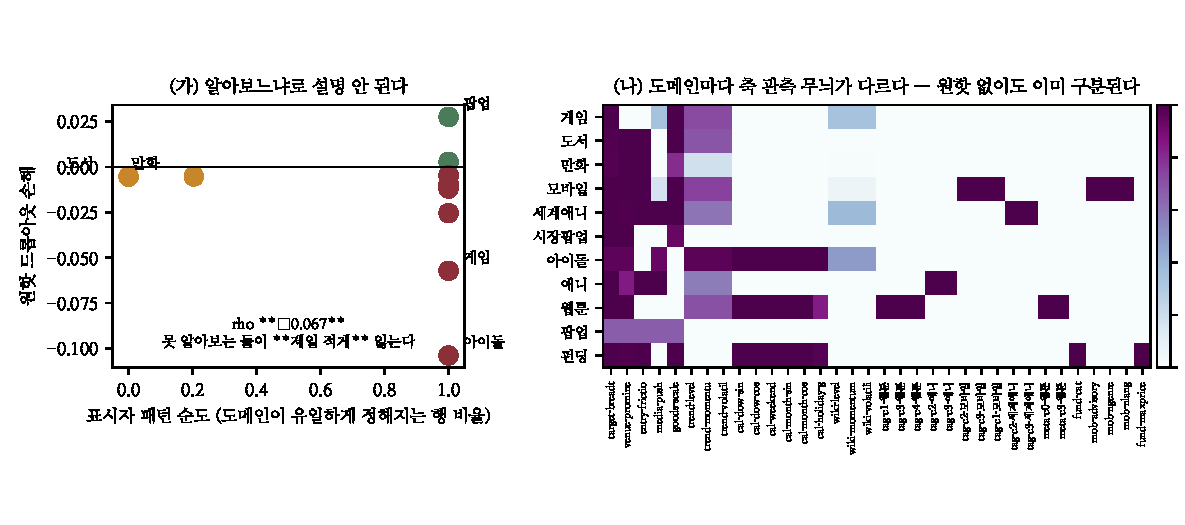
\includegraphics[width=\textwidth]{figs/fig404.pdf}
\caption{(가) 표시자 무늬 순도와 원핫 드롭아웃 손해는 관계가 없다
($\rho = -0.067$) --- 정보를 못 주는 도서·만화가 오히려 제일 적게 잃는다.
(나) 도메인 $\times$ 축의 관측 표시자 평균. 가진 축의 집합이 도메인마다
달라 무늬가 곧 이름표다. 겹치는 것은 도서와 만화뿐.}
\end{figure}

\end{document}
